
\chapter{Framework in Theory}\label{chapter:Foundation}
In this chapter we explain the framework model in theory, the key concepts behind it, challenges facing the design and their possible solutions.


\section{Foundation}
	The fundamental core element of this framework is the computational unit, which is responsible for describing the use case. One possible abstraction of the computational unit is the \textit{flow}, which is a purposeful unit of computation that contains sequentially meaningful instructions. Also, it can be either standalone self-contained computation or interactive in which they collaborate with other flows for data gathering, sharing and processing. Moreover, the flow is composed of elements which could have a significant meaning such as snapping a photo or could act as an intermediary to harmonize data as shown in figure \ref{fig:flow}. 
	
\begin{figure}[H]
	\centering
	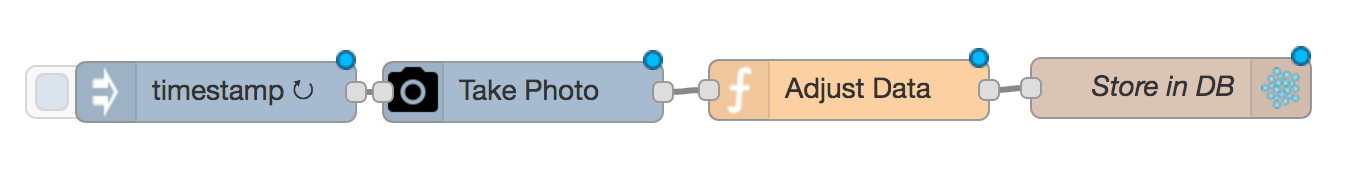
\includegraphics[scale=0.5]{images/db-out.png} 
	\caption{A node-red flow that stores an image in a database every time interval}
	\label{fig:flow}
\end{figure}

After having defined flows, it is important to give an idea on how they end up being executed. To begin with, we must address the challenge that flows are distributed in the sense that each flow could reside on different node. In addition, as previously mentioned, flows may be interactive, therefore, they need a way to communicate through distributed systems. Moreover, since nodes might be disconnected,  the communication mechanism must guarantee that there  exit  a way  in which data could be transfered between these disconnected nodes. Furthermore, it  should handle sending the computations themselves from one node to another, at the end we would like to be pervasive and manage sending computations everywhere.

 Another challenge that faces the flows execution, is the dependencies and resources which could be demanded in order to carry on the execution. They vary from one use case to another, thus needs to be orchestrated across nodes through messaging system.

Now assuming that we can send flows to the nodes, make them communicate and care for their dependencies and resources, one aspect remains, which is triggering the execution of flows. There are multiple ways to start carrying on an execution, one simple example is a time interval trigger as shown in \ref{fig:flow}. Other ways include, starting computation execution when new incoming data has been received or other events have been triggered.\\




 A flow should be modular having a specific functionality with defined interfaces that helps in reducing the complexity, allowing re-use and re-assembly. Moreover, since flows need to interact and exchange data, they should be composable. Think of composability as LEGO parts that need to be assembled in their correct positions in order to create a figure, however in contrast to individual LEGO parts which do not have a meaning on their own, individual flow elements could serve a specific purpose besides their global one. To establish flow composability in our context, we need to be able to match the output data of one flow to the input data of another, no matter whether the flows are on the same node or distributed, connected or disconnected. For instance in general terms, if we have a flow \(f_1\) that takes \(A\) as input and gives \(B\) as an output
\[ f_1 : A  \to B  \]
then we have another flow \(f_2\) that takes \(B\) as an input and gives a new output \(C\)
% the output of \(f_1\) and produce a new result and so on. 
\[ f_2 : B  \to C  \]
we should be able to compose a new flow taking \(f_1\)'s input and giving \(f_2\)'s output, resulting in flow \(f_3\) which is a composite of both.
\[f_3: A \to C = f_2 \circ f_1\]
Since composability should also be valid in a local or distributed environment. Thus, in the first case of local flow composability, there should be a way to connect the output of a flow to the input of another as shown in \ref{fig:compose}. On the other hand if it is distributed composability, the messaging system should connect the dots and serve as a broker to deliver the data.

\[a \in A, \, b \in B, \, c \in C\]
\begin{figure}[H]
	\centering
	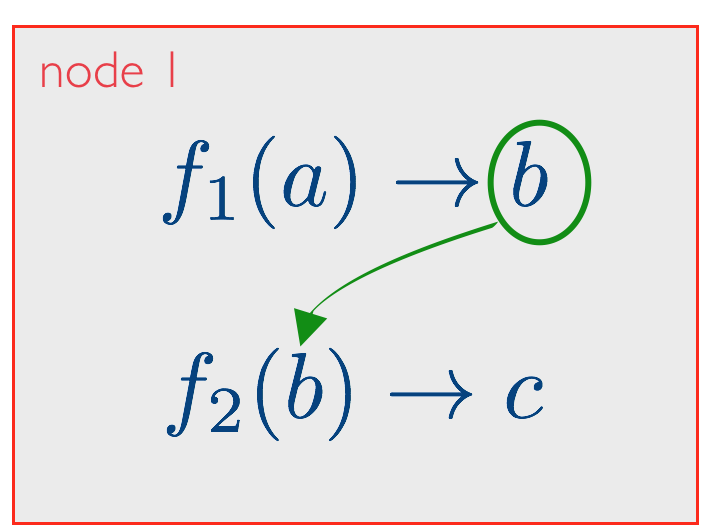
\includegraphics[scale=0.3]{images/local-compose.png} 
 	\caption{A node containing two composable flows}
	\label{fig:compose}
\end{figure}
\begin{figure}[H]
	\centering
	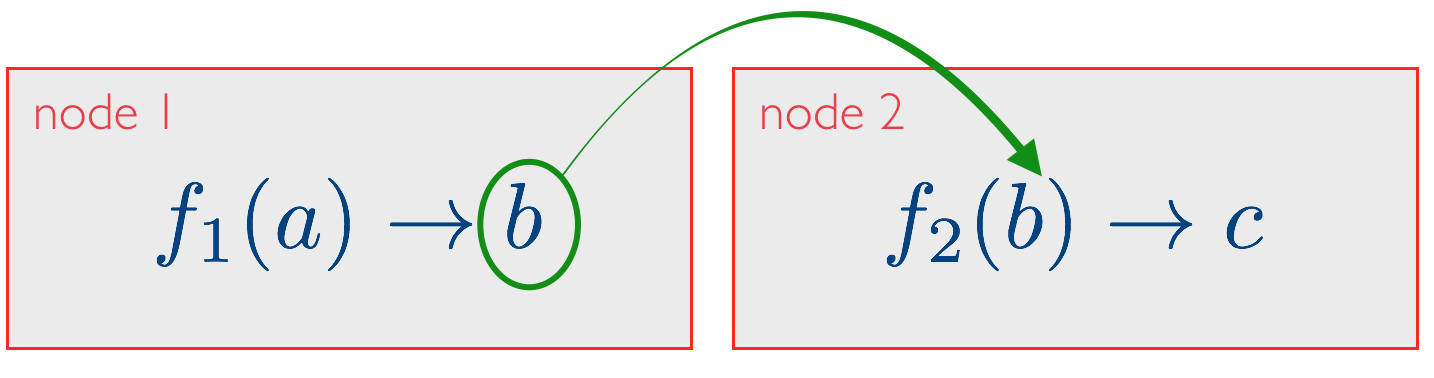
\includegraphics[scale=0.4]{images/distributed-compose.png}
	\caption{Two separate nodes having distributed composability}
	\label{fig:compose2}
\end{figure}


\section{Computational Model}

Below we present the computational model as an abstraction for the framework design, it explains the components, challenges and the possible solutions that could be implemented to overcome these challenges. 	

\subsection{Distributed Nodes \& Flows}
In order to start with the framework explanation we must understand the idea behind pervasiveness. Pervasive computing relies on the idea of pushing flows to the edges "nodes" and thus it is fundamentally distributed. A system is distributed if its components  are on networked computers which communicate only by sending and receiving of messages \cite{DSYS} which is exactly the case. Now in our model, each node should be capable of executing flows and producing results as long as it  has the required dependencies and resources. Moreover, to ensure that flows are composable, nodes should be able to communicate seamlessly even though nodes hosting this flows might be disconnected.


% Thus to have distributed nodes, we need to make sure of the following: \textit{(i)} dependencies and resources are available on the node, \textit{(ii)} there is a way to communicate between nodes,  \textit{(iii)} we can overcome sending and receiving data between disconnected nodes.  \\

Turning to flows, in essence every challenge related to making the nodes distributed also apply to flows because nodes host flows. However, there are more to flows, distributing them across nodes could have different semantics and approaches depending on the use case.
 Lets us first consider the two different semantics, a flow could be sent on random basis to the nodes, and at the contrary, it could also be sent to specific nodes. This provides flexibility in applying the use case without wasting resources, in addition, it magnifies the effect of locational context in case we want to send a computation to a specific place.
 Moving on to approaches, a flow could be distributed across the nodes in a multiple ways explained as follows: (i) flows are pushed to all the available nodes even if they are disconnected (ii) flows are sent to \textit{n} number of nodes whether they are selected or picked at random, (iii) choosing only one node to execute a specific flow. As a result, the communication model is one of the most crucial parts to guarantee a distributed system, it should have the flexibility to provide these approaches and overcome the hurdle of disconnected nodes.
 

Another main challenge is to actually find the connected nodes. Distributed and pervasive environments are dynamic, their components are not known to be live or dead at compile-time. Thus the framework should be able to run service discovery at run-time in order to find the connected nodes or it should be able to broadcast its message to all the other nodes and receive them as well. Otherwise, the approach would not qualify to be a distributed system. 




\newpage

\subsection{Pub-Sub Messaging Queues}

As previously stated, a smart communication system is essential to our computational model, it solves some of the biggest challenges in our approach which are mainly nodes service discovery, sending and receiving messages of distributed, connected and disconnected nodes. Also, considering that service discovery is dynamic, the communications model is not end-point centric since we cannot target the actual nodes as end points. The reason for that is, we do not know their respective addresses or either they are connected or not. Rather our communication model is data-centric meaning it knows that there are some parties interested in sending data and others willing to revive the same data given the same context regardless their network location.
For all the stated facts, publish-subscribe messaging queues would best fit our needs. It implements service discovery, hence, it can discover all the other nodes who has the 



\newpage


\subsection{Dependencies}

Dependencies are one of the main requirements of computation execution, dropping one or more dependency would definitely stop the execution from proceeding. Thus, we need to deal with them and make sure they do not introduce any impediments during execution.  There are two types of dependencies; the static software frameworks that the whole design relies on and must exist on each node, and the dynamic dependencies that are specific to each computation.

First, are the static dependencies are mainly the common libraries and software that most of the computations would require, they represent the base of framework. That is why these dependencies are installed to each node in our design, examples of these dependencies include the operating system, data store and any other standard or custom libraries that are mandatory for the computation to run. In addition to, the messaging system which implements the communication model allowing interaction between nodes. 

 Second, are the dynamic dependencies which are specific to each computation such as additional scripts, configuration files or libraries. In this case, they cannot be installed at node initialization since we can not know what are the custom dependencies any computation would need beforehand. Therefore, the computational model design should allow a way to configure additional dependencies. Moreover, the communication mechanism should support this configuration and grant a way to carry the configured dependencies forward to other nodes.
 
 
  Dynamic dependencies creates a bit of ambiguity, suppose that the dependency which is being sent by means of the communication mechanism is already on the receiving node. This introduces a  versioning problem, also what makes it more complicated, is that the node does not know if it possesses an older version of the dependency or a newer one. Furthermore,  imagine there is a computation on the node that uses an older version of the same library while the maintainer is sending a new computation with a newer version of the same library that is not backward compatible. 
  
   Nevertheless, there are multiple possible solutions to remove the ambiguity and make the custom dependency shipping more concrete; one solution would be to give the dependencies different names according to their versions before shipping them, hence, any different version would not replace the existing ones. Another solution would be to design a system that links each running computation on the node to its dependencies and once a collision appears, the new computation renames its dependency and uses the renamed one.
 

\subsection {Resources}


Resources are a different type of dependency which are also necessary for computations to run. However, they might differ or not exist at all on each node. If one of the needed resources is missing then the computation could be either dismissed or queued depending on the type of resource. Moreover, the maintainers cannot make any assumptions about the resources, meaning, an assumption stating that each node has a camera is not necessarily true. Since the resources cannot be standardized across all nodes, each computation must provide meta data expressing the resources it is going to require, also, the node must realize its available resources. Then a node can check against its capabilities and decide whether it could carry out the execution or not. There are two types of resources; sensors and actuators which are used throughout a computation, and the hardware resources which influences the performance requirements of a specific computation.


\subsubsection{Sensors and Actuators}

  Sensors and actuators are resources attached to a node such as cameras, temperature and gas sensors. Executing a computation missing this type of resource on a node should have a lower possibility of being queued, since its highly unlikely that this hardware resource would be attached soon. A node should be aware of its available resources, otherwise, it would not be able to compare the requirements of incoming computations against its capabilities. Hence one possible solution, is for each node to have a specification file as a static dependency stating its available resources.
  
  However sensors and actuators are dynamic, they can be added or removed on demand, therefore, having them in a specification file as a static dependency which is only set at initialization time will be troublesome. Of course, we can always edit the specification file once we change the state of any of these resources, but this solution is not very efficient nor scalable, as it increases the manual work. It would be much easier if the node could run resource discovery to find its attached resources each time it receives a computation.
  
  Moving on to consider computations acquiring the same resource at the same time, for instance, two computations that want to take a photo at the same time. This is problematic because whichever computation acquires a lock on the camera first will succeed while the other will fail. Therefore as a resolution, we could use resource decoupling; instead of having the computation ask a specific resource directly for information, the  data will be pushed into a database. Afterwards, the different computations could query the data from a database.
  
  

\subsubsection{Hardware Resources }

The second type of resources is related to the node performance, its power and memory capabilities, it is heavily biased by the processor of the node and its random access memory type and size. Computations vary in terms of resource consumption and hence a heavy computation should not be deployed to a node which is already loaded. 

Considering that each computation model has meta-data describing its resource consumption, then it is possible to decide if it is going to be deployed on a specific node or not. Additionally, if it is not going to be deployed then it should be decided whether the computation is going to be queued or dismissed according to the possibility of acquiring the resource.

The idea of queuing computations however develops a scheduling problem. Since we have a queue of computations inside each node, we will have a race condition on which computation should be deployed first according to available resources. Furthermore, since some computations might be dismissed, a rather bigger scheduling problem will come up when we try to fit the all computations across nodes in the whole system framework 
\newpage




\section{Data Model}

\subsection{Data Types}
%we can ask the high performance units to stream from cameras no low devices. but how to do it ?

%\subsection{Explain data distribution among several nodes to apply pervasive computing}

\subsection{Moving Data}

% moreover, the way that the input data used while doing this computation will be provided, whether it gets the input data from a local database or is it going to be included along with the computational data. 
\subsection{IO Specification}
- I/O spec design for databases for two composable flows


\section{System Design }
A System Design can be broadly described as an architecture of the system, which includes an explanation of each and every hardware component of the system, the connection between these components if there is any, and the data flowing between these components. Moreover, it provides a wide glimpse of the whole system but not its exact functionality, hence, giving a simple understanding of the architecture without jumping into much detail.\\
Initially, the components of the System Design is introduced, then, the connection between these components is shown, and eventually, the flow of the data is pointed out.

\subsection{Components}
\label{sub:components}
Below, each component of the proposed system design is explained.

\subsubsection{Node}
\label{subsub:node}
%The first set of components to explain are the sensors, they refer to objects that detect certain change in the environment and converts these changes into digital data and 
%which refer to objects that can detect certain changes in the environment and converts them to digital data, 
A Node is one of the core components of this design, it is a small computer device of low storage and computation capacity compared to nowadays portable computers, commonly a \textit{Raspberry Pi} but could be any other device. It is connected to several sensors which typically detect certain changes in the environment and converts it into digital data, for instance, Gas sensor, Temperature sensor or a Camera. Then, the device either stores the data into a local database, performs a computation locally, does both or even asks other nodes to do computation instead, however, an assumption about which sensors or specifications does a specific node  possess can not be made, meaning, each node might not have the exact number or types of sensors because each node may be deployed in a different timing or context. Thus, each node has a configuration file specifying its capabilities. A typical node is shown in figure \ref{fig:node}

\begin{figure}[H]
\centering
 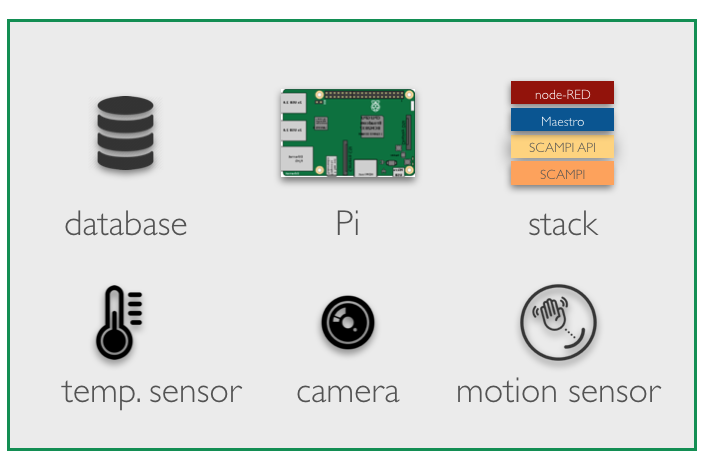
\includegraphics[scale=0.4]{images/node.png}
 \caption{A typical node in the system}
 \label{fig:node}
\end{figure}

\subsubsection{High Performance  Units }

CPUs in the proposed system nodes in \ref{subsub:node}. An example of a high processing unit is  a Graphics Processing unit \textit{GPU}.

\begin{figure}[H]
	\centering
	
\includegraphics[scale=0.7]{images/gpu.png}
		\caption{Figure denoting a Graphics Processing Unit GPU}
	\label{fig:gpu}
\end{figure}

\subsubsection{Network}
\label{subsub:network}
A Network in this design is a set of connected components which are capable of communicating and therefore allowing data sharing between them.
\begin{figure}[H]
	\centering
	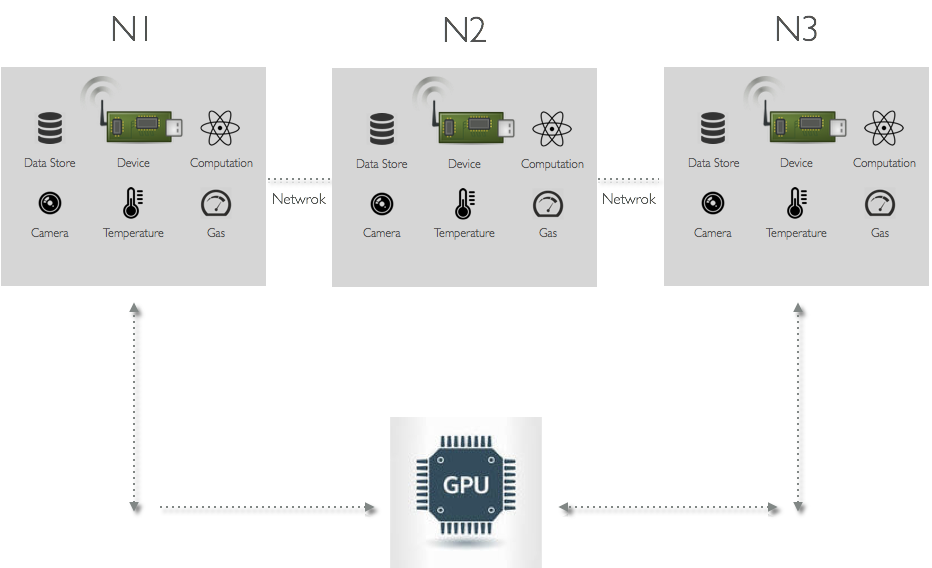
\includegraphics[scale=0.4]{images/network.png}
	\caption{A network consisting of three connected nodes and a GPU}
	\label{fig:network}
\end{figure}
-- TODO: 
Emphasis the difference between persistent and non persistent network links in system design.

\subsubsection{Mobile Device}
A Mobile Device in this context is any device that can connect to the network containing the nodes and is allowed to  carry data from one network to another, hence, allowing a form of data sharing between networks or nodes which are not connected.

\begin{figure}[H]
	\centering
	
\includegraphics[scale=0.3]{images/mobile.png}
	\caption{Figure denoting a Mobile Device}
	\label{fig:mobile}
\end{figure}



\subsection{Connectivity and Data Flow}
A Network described in \ref{subsub:network}, is a simple form of connectivity between components, however, components and specifically nodes are not necessarily connected, sometimes they are just a standalone component that cannot share any information via direct connectivity, also, networks could be disconnected as well, meaning, a network might not be connected to the whole system, thus, is a standalone network. In these cases, a mobile device could help in carrying information and data between these disconnected nodes or networks. 

\begin{figure}[H]
	\centering
	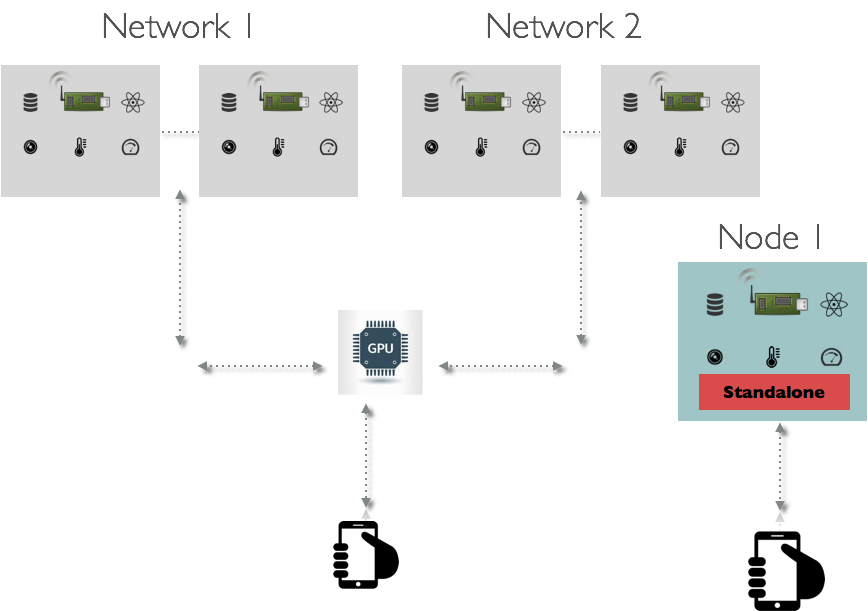
\includegraphics[scale=0.5]{images/system.png}
	\label{fig:system}
	\caption{Two networks connected with a GPU and one standalone network}
\end{figure}









\section{Summary}



